% Options for packages loaded elsewhere
% Options for packages loaded elsewhere
\PassOptionsToPackage{unicode}{hyperref}
\PassOptionsToPackage{hyphens}{url}
\PassOptionsToPackage{dvipsnames,svgnames,x11names}{xcolor}
%
\documentclass[
]{article}
\usepackage{xcolor}
\usepackage[margin=1in]{geometry}
\usepackage{amsmath,amssymb}
\setcounter{secnumdepth}{5}
\usepackage{iftex}
\ifPDFTeX
  \usepackage[T1]{fontenc}
  \usepackage[utf8]{inputenc}
  \usepackage{textcomp} % provide euro and other symbols
\else % if luatex or xetex
  \usepackage{unicode-math} % this also loads fontspec
  \defaultfontfeatures{Scale=MatchLowercase}
  \defaultfontfeatures[\rmfamily]{Ligatures=TeX,Scale=1}
\fi
\usepackage{lmodern}
\ifPDFTeX\else
  % xetex/luatex font selection
\fi
% Use upquote if available, for straight quotes in verbatim environments
\IfFileExists{upquote.sty}{\usepackage{upquote}}{}
\IfFileExists{microtype.sty}{% use microtype if available
  \usepackage[]{microtype}
  \UseMicrotypeSet[protrusion]{basicmath} % disable protrusion for tt fonts
}{}
\makeatletter
\@ifundefined{KOMAClassName}{% if non-KOMA class
  \IfFileExists{parskip.sty}{%
    \usepackage{parskip}
  }{% else
    \setlength{\parindent}{0pt}
    \setlength{\parskip}{6pt plus 2pt minus 1pt}}
}{% if KOMA class
  \KOMAoptions{parskip=half}}
\makeatother
% Make \paragraph and \subparagraph free-standing
\makeatletter
\ifx\paragraph\undefined\else
  \let\oldparagraph\paragraph
  \renewcommand{\paragraph}{
    \@ifstar
      \xxxParagraphStar
      \xxxParagraphNoStar
  }
  \newcommand{\xxxParagraphStar}[1]{\oldparagraph*{#1}\mbox{}}
  \newcommand{\xxxParagraphNoStar}[1]{\oldparagraph{#1}\mbox{}}
\fi
\ifx\subparagraph\undefined\else
  \let\oldsubparagraph\subparagraph
  \renewcommand{\subparagraph}{
    \@ifstar
      \xxxSubParagraphStar
      \xxxSubParagraphNoStar
  }
  \newcommand{\xxxSubParagraphStar}[1]{\oldsubparagraph*{#1}\mbox{}}
  \newcommand{\xxxSubParagraphNoStar}[1]{\oldsubparagraph{#1}\mbox{}}
\fi
\makeatother


\usepackage{longtable,booktabs,array}
\usepackage{calc} % for calculating minipage widths
% Correct order of tables after \paragraph or \subparagraph
\usepackage{etoolbox}
\makeatletter
\patchcmd\longtable{\par}{\if@noskipsec\mbox{}\fi\par}{}{}
\makeatother
% Allow footnotes in longtable head/foot
\IfFileExists{footnotehyper.sty}{\usepackage{footnotehyper}}{\usepackage{footnote}}
\makesavenoteenv{longtable}
\usepackage{graphicx}
\makeatletter
\newsavebox\pandoc@box
\newcommand*\pandocbounded[1]{% scales image to fit in text height/width
  \sbox\pandoc@box{#1}%
  \Gscale@div\@tempa{\textheight}{\dimexpr\ht\pandoc@box+\dp\pandoc@box\relax}%
  \Gscale@div\@tempb{\linewidth}{\wd\pandoc@box}%
  \ifdim\@tempb\p@<\@tempa\p@\let\@tempa\@tempb\fi% select the smaller of both
  \ifdim\@tempa\p@<\p@\scalebox{\@tempa}{\usebox\pandoc@box}%
  \else\usebox{\pandoc@box}%
  \fi%
}
% Set default figure placement to htbp
\def\fps@figure{htbp}
\makeatother





\setlength{\emergencystretch}{3em} % prevent overfull lines

\providecommand{\tightlist}{%
  \setlength{\itemsep}{0pt}\setlength{\parskip}{0pt}}



 


\usepackage{booktabs}
\usepackage{longtable}
\usepackage{array}
\usepackage{multirow}
\usepackage{wrapfig}
\usepackage{float}
\usepackage{colortbl}
\usepackage{pdflscape}
\usepackage{tabu}
\usepackage{threeparttable}
\usepackage{threeparttablex}
\usepackage[normalem]{ulem}
\usepackage{makecell}
\usepackage{xcolor}
\usepackage{longtable}[=v4.13]
\makeatletter
\@ifpackageloaded{caption}{}{\usepackage{caption}}
\AtBeginDocument{%
\ifdefined\contentsname
  \renewcommand*\contentsname{Table of contents}
\else
  \newcommand\contentsname{Table of contents}
\fi
\ifdefined\listfigurename
  \renewcommand*\listfigurename{List of Figures}
\else
  \newcommand\listfigurename{List of Figures}
\fi
\ifdefined\listtablename
  \renewcommand*\listtablename{List of Tables}
\else
  \newcommand\listtablename{List of Tables}
\fi
\ifdefined\figurename
  \renewcommand*\figurename{Figure}
\else
  \newcommand\figurename{Figure}
\fi
\ifdefined\tablename
  \renewcommand*\tablename{Table}
\else
  \newcommand\tablename{Table}
\fi
}
\@ifpackageloaded{float}{}{\usepackage{float}}
\floatstyle{ruled}
\@ifundefined{c@chapter}{\newfloat{codelisting}{h}{lop}}{\newfloat{codelisting}{h}{lop}[chapter]}
\floatname{codelisting}{Listing}
\newcommand*\listoflistings{\listof{codelisting}{List of Listings}}
\makeatother
\makeatletter
\makeatother
\makeatletter
\@ifpackageloaded{caption}{}{\usepackage{caption}}
\@ifpackageloaded{subcaption}{}{\usepackage{subcaption}}
\makeatother
\usepackage{bookmark}
\IfFileExists{xurl.sty}{\usepackage{xurl}}{} % add URL line breaks if available
\urlstyle{same}
\hypersetup{
  pdftitle={Oklahoma Induced Seismicity: Causal ETAS Analysis},
  pdfauthor={PPDisentangle},
  colorlinks=true,
  linkcolor={blue},
  filecolor={Maroon},
  citecolor={Blue},
  urlcolor={Blue},
  pdfcreator={LaTeX via pandoc}}


\title{Oklahoma Induced Seismicity: Causal ETAS Analysis}
\usepackage{etoolbox}
\makeatletter
\providecommand{\subtitle}[1]{% add subtitle to \maketitle
  \apptocmd{\@title}{\par {\large #1 \par}}{}{}
}
\makeatother
\subtitle{Bivariate ETAS with Partition Sensitivity}
\author{PPDisentangle}
\date{2026-03-15}
\begin{document}
\maketitle

\renewcommand*\contentsname{Table of contents}
{
\hypersetup{linkcolor=}
\setcounter{tocdepth}{3}
\tableofcontents
}

\section{Introduction}\label{introduction}

\textbf{Report rendered at:} 2026-03-15 23:39:23 EDT

On 18 March 2015 the Oklahoma Corporation Commission (OCC) issued
directive \textbf{AOI\_20150318}, requiring operators within a defined
Area of Interest (AOI) in central Oklahoma to reduce wastewater disposal
volumes. This report estimates the \textbf{all-or-nothing causal effect}
of the directive on earthquake rates using the \textbf{PPDisentangle}
framework.

\subsection{Estimand}\label{estimand}

The target quantity is the \textbf{all-or-nothing total treatment
effect}: the expected difference in total earthquake counts between a
world in which \emph{every} county receives the directive
(\(\mathbf{Z}=(1,\dots,1)\)) and a world in which \emph{no} county
receives it (\(\mathbf{Z}=(0,\dots,0)\)):

\[
\Delta_{\text{AoN}}
= \bigl\{
   \mathbb{E}\!\bigl[N(\mathbf{1})\bigr]
  -\mathbb{E}\!\bigl[N(\mathbf{0})\bigr]
\bigr\},
\]

where \(N(\mathbf{z})\) denotes the total event count under treatment
assignment \(\mathbf{z}\).

\subsection{Models}\label{models}

The analysis fits four bivariate ETAS models on the \textbf{county
partition}:

\begin{longtable}[]{@{}clll@{}}
\toprule\noalign{}
Label & Model & Background & Labels \\
\midrule\noalign{}
\endhead
\bottomrule\noalign{}
\endlastfoot
\textbf{B} & Naive bivariate ETAS & Homogeneous & Location-based \\
\textbf{D} & SEM bivariate ETAS & Homogeneous & SEM-corrected \\
\textbf{E} & Naive bivariate ETAS & KDE (non-parametric) &
Location-based \\
\textbf{F} & SEM bivariate ETAS & KDE (non-parametric) &
SEM-corrected \\
\end{longtable}

Additionally, fits B and D are repeated under alternative
\textbf{partitioning schemes} to assess sensitivity to spatial
resolution.

\section{Study Design}\label{study-design}

\textbf{Treatment.} OCC directive AOI\_20150318: mandatory reduction in
wastewater disposal volumes within the AOI.

\textbf{Tessellation.} The 77 Oklahoma counties (US Census Bureau via
\texttt{tigris}). Counties whose centroid falls inside the AOI are
treated.

\textbf{Treated counties} (9): Pawnee, Love, Alfalfa, Oklahoma, Logan,
Payne, Noble, Grant, Lincoln.

\textbf{Temporal windows.}

\begin{itemize}
\tightlist
\item
  Pre-treatment: 2014-01-01T00:00:00Z to 2015-03-18T00:00:00Z
\item
  Post-treatment: 2015-03-18T00:00:00Z to 2015-06-24T00:00:00Z
\end{itemize}

\textbf{Magnitude threshold.} \(m_0 =\) 2.5.

\textbf{Event counts.} - Pre-treatment total: 2472 - Pre-treatment
holdout (first 50\%): 1236 - Pre-treatment used for estimation/carryover
(second 50\%): 1236 - Post-treatment: 818 - Total used in SEM estimation
(used pre + post): 2054

\section{Data}\label{data}

\subsection{Magnitude Distribution}\label{magnitude-distribution}

\begin{figure}

\centering{

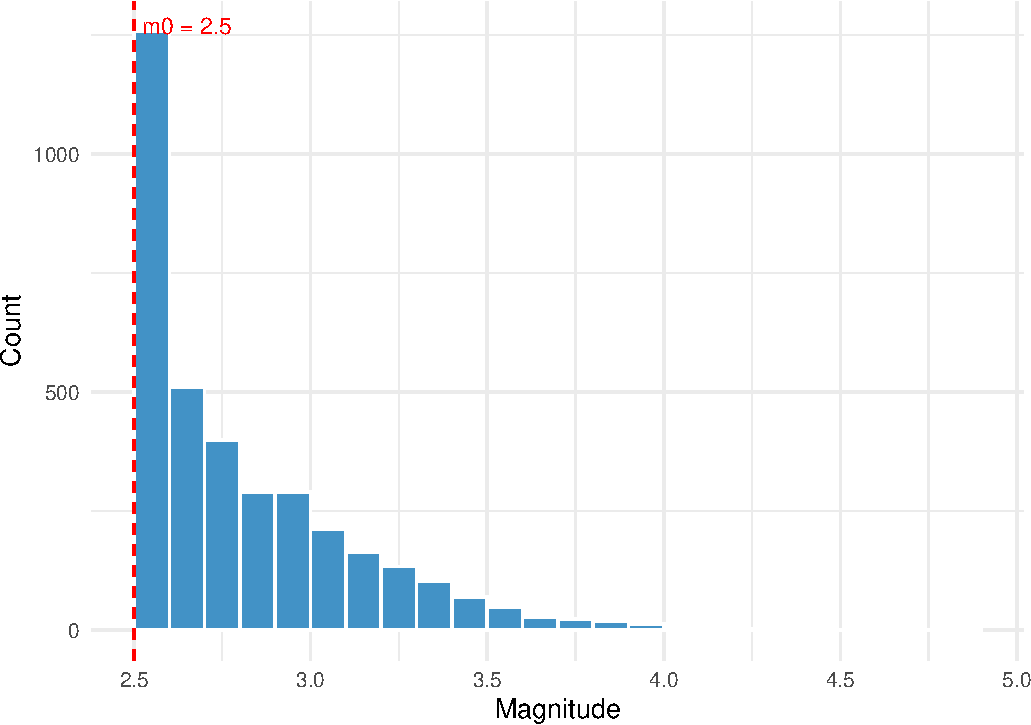
\includegraphics[width=1\linewidth,height=\textheight,keepaspectratio]{oklahoma_report_files/figure-pdf/fig-mag-1.pdf}

}

\caption{\label{fig-mag}Magnitude distribution of events above the
completeness threshold.}

\end{figure}%

\subsection{Temporal Profile}\label{temporal-profile}

\begin{figure}

\centering{

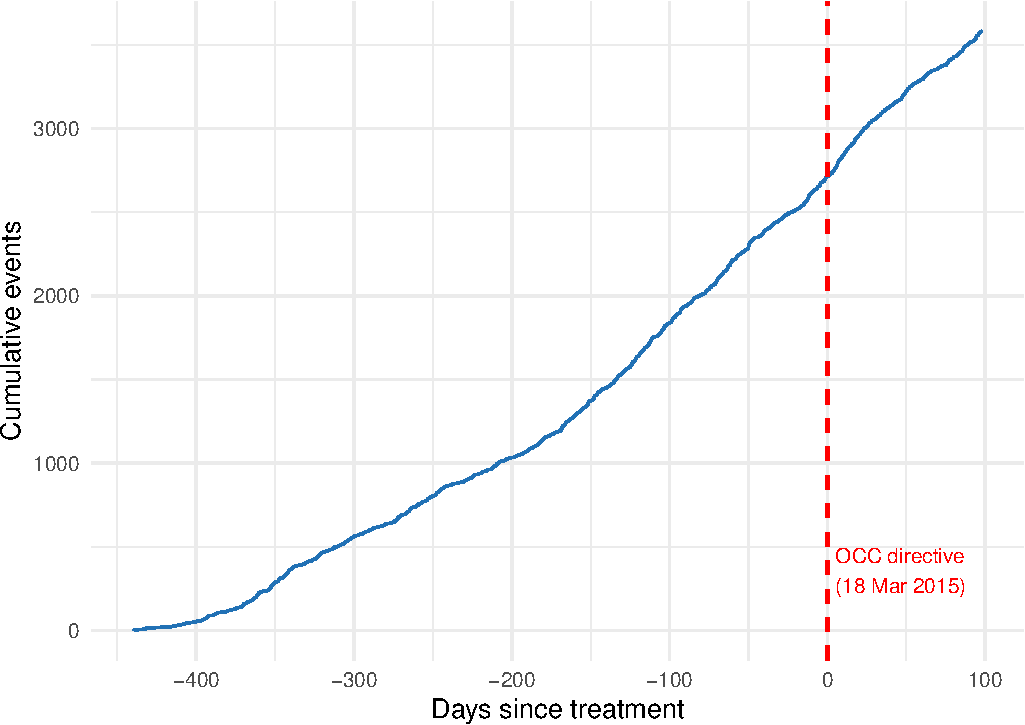
\includegraphics[width=1\linewidth,height=\textheight,keepaspectratio]{oklahoma_report_files/figure-pdf/fig-temporal-1.pdf}

}

\caption{\label{fig-temporal}Cumulative event count; dashed line marks
the OCC directive.}

\end{figure}%

\subsection{County Partition}\label{county-partition}

\begin{figure}

\centering{

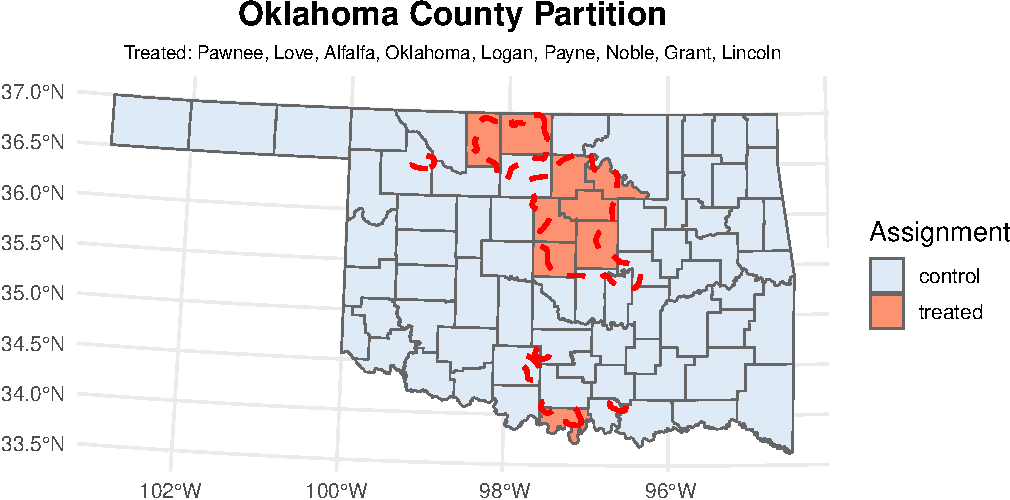
\includegraphics[width=1\linewidth,height=\textheight,keepaspectratio]{oklahoma_report_files/figure-pdf/fig-partition-1.pdf}

}

\caption{\label{fig-partition}Oklahoma county-level partition. Red
counties are treated (centroid inside AOI).}

\end{figure}%

\subsection{Point Patterns}\label{point-patterns}

\begin{figure}

\centering{

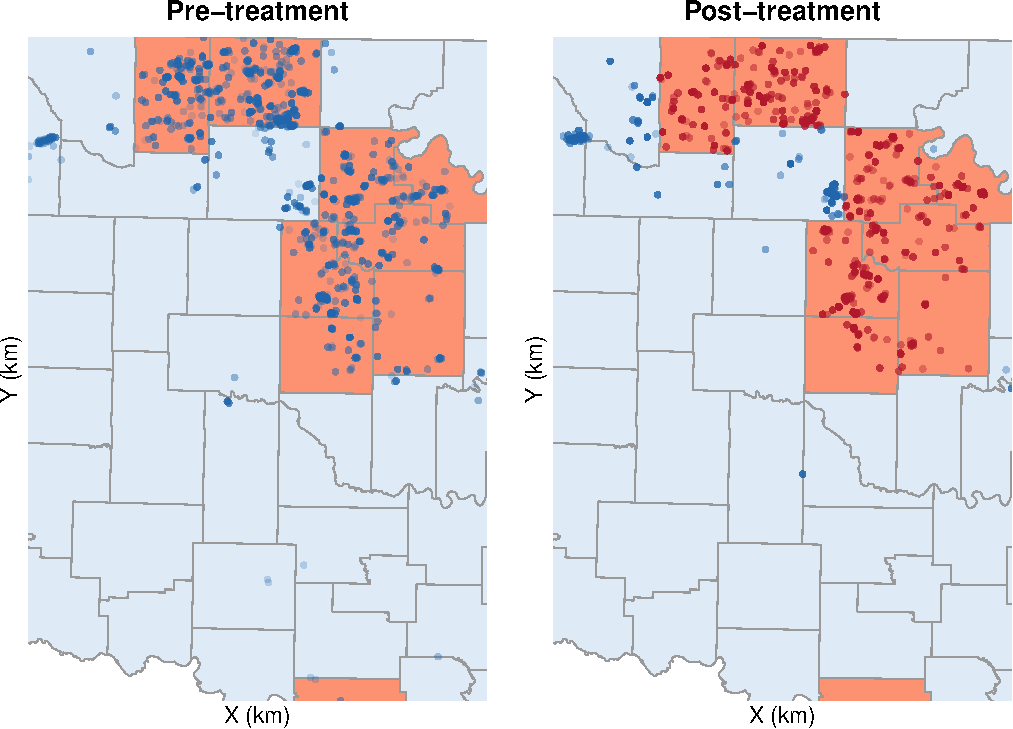
\includegraphics[width=1\linewidth,height=\textheight,keepaspectratio]{oklahoma_report_files/figure-pdf/fig-pp-1.pdf}

}

\caption{\label{fig-pp}Pre-treatment (left) and post-treatment (right)
events overlaid on the county partition.}

\end{figure}%

\section{Model}\label{model}

\subsection{ETAS Conditional
Intensity}\label{etas-conditional-intensity}

\[
\lambda(t,x,y) = \frac{\mu}{|S|} + \sum_{j:\,t_j<t} A\,e^{\alpha_m(m_j-m_0)}\,g(t-t_j)\,f(x-x_j,y-y_j\mid m_j)
\]

with Omori--Utsu temporal kernel \(g\) and power-law spatial kernel
\(f\).

\subsection{Bivariate Extension}\label{bivariate-extension}

\[
\lambda_k(t,x,y) = \frac{\mu_k}{|S_k|}\,W_k(x,y) + \sum_{l\in\{0,1\}}\sum_{\substack{j:\,t_j<t\\Z_j=l}} A_{kl}\,e^{\alpha_{m,kl}(m_j-m_0)}\,g(t-t_j)\,f(x-x_j,y-y_j\mid m_j)
\]

Off-diagonal terms \(A_{01}\) (treated\(\to\)control) and \(A_{10}\)
(control\(\to\)treated) capture cross-excitation. For the KDE background
models (E, F), \(W_k(x,y)\) is the normalized kernel density estimate
from control pre-treatment data; for the homogeneous models (B, D),
\(W_k \equiv 1\).

\subsection{Non-Parametric Background
Rate}\label{non-parametric-background-rate}

\begin{longtable}[t]{lc}

\caption{\label{tbl-kde}KDE background rate estimation details.}

\tabularnewline

\\
\toprule
Setting & Value\\
\midrule
KDE training events (held-out control pre) & 124\\
Held-out pre-treatment events (all processes) & 1236\\
Pre-treatment events used for estimation & 1236\\
Bandwidth (km) & 1.57\\
Estimated triggering range (km) & 4.89\\
\addlinespace
Method & Diggle cross-validation\\
\bottomrule

\end{longtable}

Only the \textbf{second 50\%} of pre-treatment events are used for
estimation/carryover in both homogeneous and inhomogeneous SEM fits. The
\textbf{first 50\%} is held out for fairness; in the inhomogeneous case,
its control events are used to estimate the KDE background via
\texttt{bw.diggle}.

\begin{figure}

\centering{

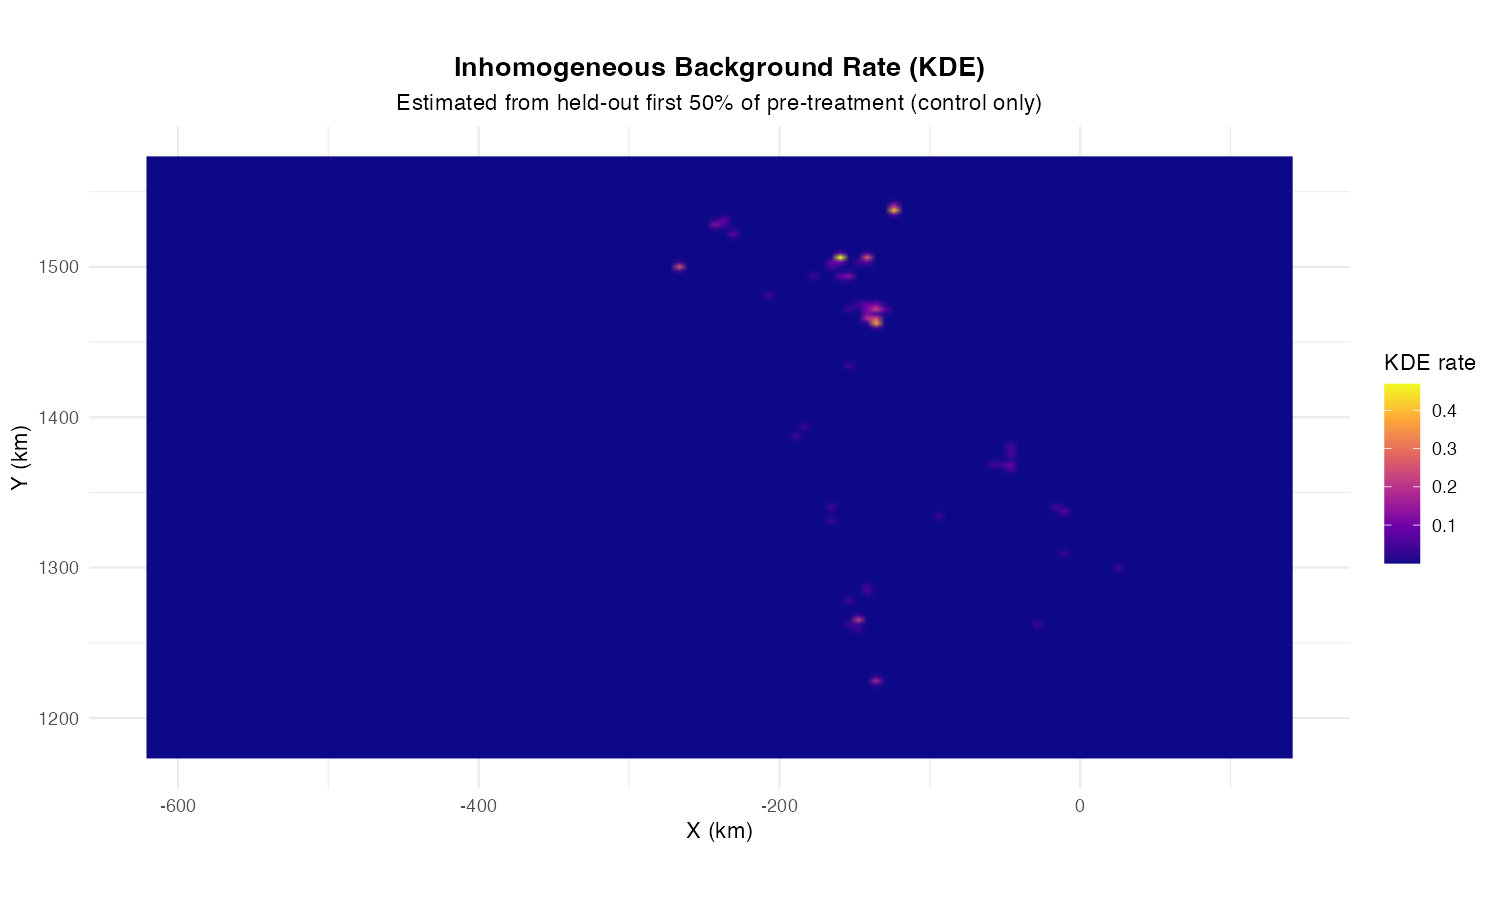
\includegraphics[width=1\linewidth,height=\textheight,keepaspectratio]{../../output/plots/background_rate_kde.png}

}

\caption{\label{fig-kde-bg}Estimated inhomogeneous background rate from
held-out control pre-treatment events.}

\end{figure}%

\subsection{Fixed Parameters}\label{fixed-parameters}

\begin{longtable}[t]{lcl}

\caption{\label{tbl-fixed}Fixed structural parameters.}

\tabularnewline

\\
\toprule
Parameter & Value & Role\\
\midrule
c & 0.05 & Omori onset delay\\
p & 1.20 & Omori decay exponent\\
D & 5.00 & Spatial scale\\
γ & 0.50 & Mag-spatial scaling\\
q & 1.50 & Spatial decay exponent\\
\bottomrule

\end{longtable}

\subsection{SEM Configuration}\label{sem-configuration}

\begin{itemize}
\tightlist
\item
  \textbf{Outer iterations:} 1
\item
  \textbf{Inner iterations:} 1000
\item
  \textbf{SEM inner proposals (\texttt{SEM\_INNER\_PROPS}):} 20
\item
  \textbf{SEM labellings (\texttt{SEM\_N\_LABELLINGS}):} 30
\item
  \textbf{Change factor:} 0.01
\end{itemize}

\section{Results --- County Partition}\label{results-county-partition}

\subsection{Marginal Parameters}\label{marginal-parameters}

\begingroup\fontsize{8}{10}\selectfont

\begin{longtable}[t]{lcccccccc}

\caption{\label{tbl-params}Marginal ETAS parameters across available
bivariate fits.}

\tabularnewline

\\
\toprule
\multicolumn{1}{c}{ } & \multicolumn{2}{c}{B: Naive Biv} & \multicolumn{2}{c}{D: SEM Biv} & \multicolumn{2}{c}{E: Naive+KDE} & \multicolumn{2}{c}{F: SEM+KDE} \\
\cmidrule(l{3pt}r{3pt}){2-3} \cmidrule(l{3pt}r{3pt}){4-5} \cmidrule(l{3pt}r{3pt}){6-7} \cmidrule(l{3pt}r{3pt}){8-9}
 & B:ctrl & B:treat & D:ctrl & D:treat & E:ctrl & E:treat & F:ctrl & F:treat\\
\midrule
\$\textbackslash{}mu\$ & 0.0247 & 1.3027 & 0.0227 & 0.2011 & 1.8886 & 0.3697 & 0.0195 & 0.1388\\
\$A\$ & 1.1569 & 0.7536 & 1.1216 & 1.0351 & 0.4953 & 0.9531 & 1.1353 & 1.0506\\
\$\textbackslash{}alpha\_m\$ & 0.3895 & 0.8682 & 0.6670 & 0.5876 & -3.1600 & 0.8654 & 0.4686 & 0.6725\\
\bottomrule

\end{longtable}

\endgroup{}

\subsection{Cross-excitation}\label{cross-excitation}

\begin{longtable}[t]{lcccc}

\caption{\label{tbl-cross}Cross-excitation parameters for available
models.}

\tabularnewline

\\
\toprule
 & B: Naive & D: SEM & E: Naive+KDE & F: SEM+KDE\\
\midrule
\$A\_\{01\}\$ (treat\$\textbackslash{}to\$ctrl) & 0.0031 & 0.0049 & 0.0565 & 0.0100\\
\$\textbackslash{}alpha\_\{m,01\}\$ & -0.0308 & 0.5123 & -1.0704 & 0.5706\\
\$A\_\{10\}\$ (ctrl\$\textbackslash{}to\$treat) & 0.0000 & 0.0160 & 0.0000 & 0.0100\\
\$\textbackslash{}alpha\_\{m,10\}\$ & -0.3251 & 0.5445 & 1.4226 & 0.5706\\
\bottomrule

\end{longtable}

\subsection{Parameter Comparison}\label{parameter-comparison}

\begin{figure}

\centering{

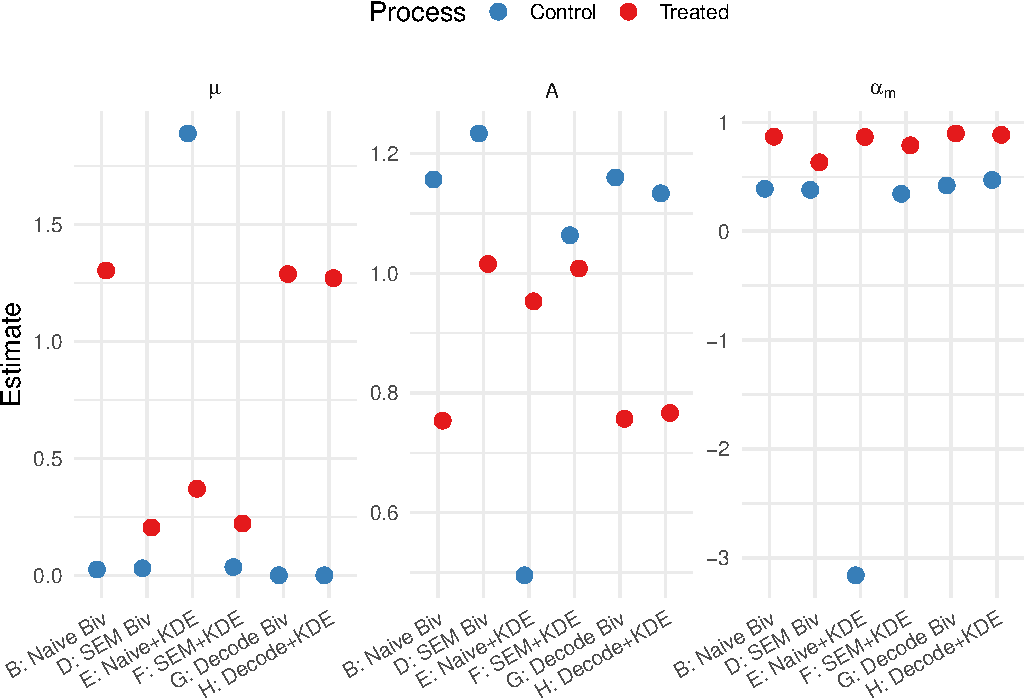
\includegraphics[width=1\linewidth,height=\textheight,keepaspectratio]{oklahoma_report_files/figure-pdf/fig-params-1.pdf}

}

\caption{\label{fig-params}Marginal parameter estimates across bivariate
fits.}

\end{figure}%

\subsection{SEM Convergence}\label{sem-convergence}

\begin{figure}

\centering{

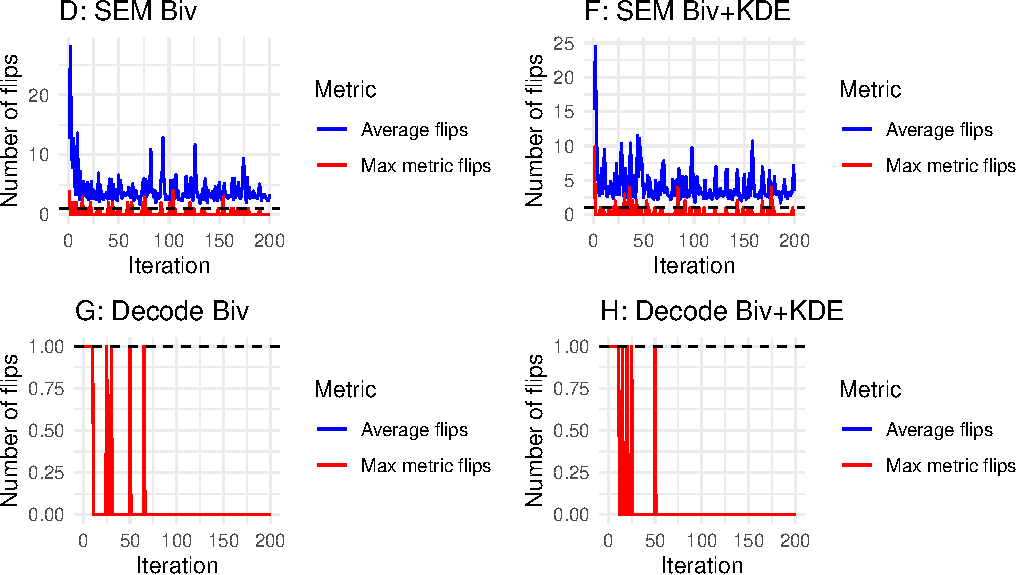
\includegraphics[width=1\linewidth,height=\textheight,keepaspectratio]{oklahoma_report_files/figure-pdf/fig-flips-1.pdf}

}

\caption{\label{fig-flips}Label flips per relabelling iteration.}

\end{figure}%

\begin{figure}

\centering{

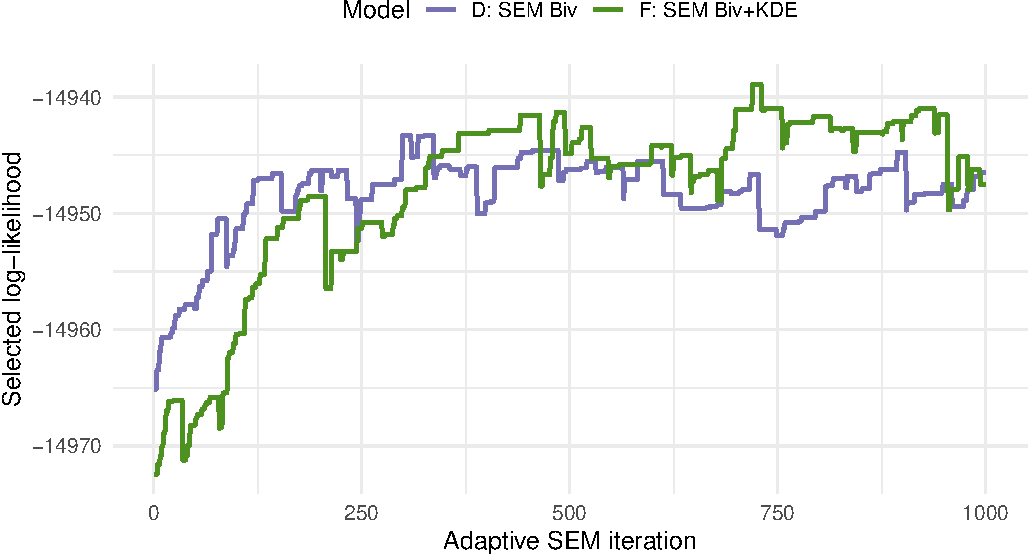
\includegraphics[width=1\linewidth,height=\textheight,keepaspectratio]{oklahoma_report_files/figure-pdf/fig-sem-adaptive-loglik-1.pdf}

}

\caption{\label{fig-sem-adaptive-loglik}Adaptive SEM selected-label
log-likelihood progression (county SEM fits).}

\end{figure}%

\subsection{SEM Relabelling: Confusion
Matrices}\label{sem-relabelling-confusion-matrices}

\subsubsection{Fit D --- SEM Bivariate
ETAS}\label{fit-d-sem-bivariate-etas}

\begin{longtable}[t]{lcc}

\caption{\label{tbl-cm-D}Fit D: Location vs SEM-inferred label (n = 818
post-treatment events).}

\tabularnewline

\\
\toprule
\multicolumn{1}{c}{Location ↓ / Inferred →} & \multicolumn{2}{c}{ } \\
\cmidrule(l{3pt}r{3pt}){1-1}
 & control & treated\\
\midrule
control & 216  (26.4\%) & 1  (0.1\%)\\
treated & 125  (15.3\%) & 476  (58.2\%)\\
\bottomrule

\end{longtable}

\subsubsection{Fit F --- SEM Bivariate + KDE
Background}\label{fit-f-sem-bivariate-kde-background}

\begin{longtable}[t]{lcc}

\caption{\label{tbl-cm-F}Fit F: Location vs SEM-inferred label (n = 818
post-treatment events).}

\tabularnewline

\\
\toprule
\multicolumn{1}{c}{Location ↓ / Inferred →} & \multicolumn{2}{c}{ } \\
\cmidrule(l{3pt}r{3pt}){1-1}
 & control & treated\\
\midrule
control & 216  (26.4\%) & 1  (0.1\%)\\
treated & 143  (17.5\%) & 458  (56\%)\\
\bottomrule

\end{longtable}

\subsubsection{Fit G --- Decode Bivariate
ETAS}\label{fit-g-decode-bivariate-etas}

\subsubsection{Fit H --- Decode Bivariate + KDE
Background}\label{fit-h-decode-bivariate-kde-background}

\subsubsection{Relabelling Summary}\label{relabelling-summary}

\begin{longtable}[t]{lccccc}

\caption{\label{tbl-cm-summary}Summary of SEM relabelling across
models.}

\tabularnewline

\\
\toprule
Model & Post events & Ctrl to Treat & Treat to Ctrl & Total relabelled & Pct relabelled\\
\midrule
D: SEM Bivariate & 818 & 1 & 125 & 126 & 15.4\%\\
F: SEM Bivariate+KDE & 818 & 1 & 143 & 144 & 17.6\%\\
\bottomrule

\end{longtable}

\section{All-or-Nothing Treatment
Effect}\label{all-or-nothing-treatment-effect}

\subsection{County Partition}\label{county-partition-1}

\begin{longtable}[t]{lccccc}

\caption{\label{tbl-ate-biv}All-or-nothing total effect over 100 days.}

\tabularnewline

\\
\toprule
Model & E[N(0)] & E[N(1)] & Total Effect / 77 counties / 100d & SD & Spillover / 100d\\
\midrule
B: Naive Bivariate & 57 & 819 & 762 & 226 & 0\\
D: SEM Bivariate & 1114 & 407 & -707 & 3218 & 1\\
E: Naive Biv+KDE & 220 & 3787 & 3567 & 3436 & 0\\
F: SEM Biv+KDE & 22 & 686 & 663 & 748 & 1\\
\bottomrule

\end{longtable}

\begin{figure}

\centering{

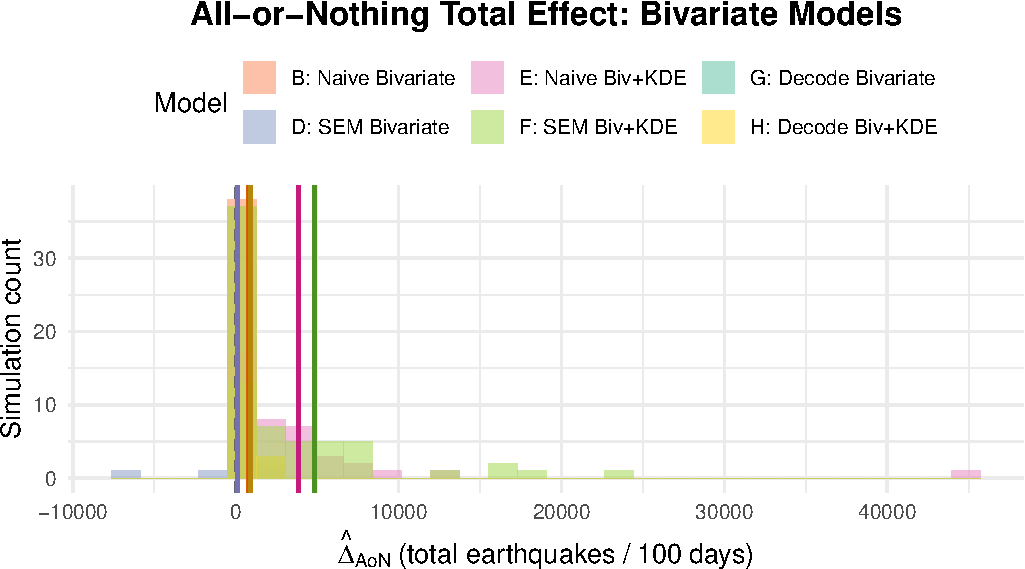
\includegraphics[width=1\linewidth,height=\textheight,keepaspectratio]{oklahoma_report_files/figure-pdf/fig-ate-biv-1.pdf}

}

\caption{\label{fig-ate-biv}Simulation distribution of the
all-or-nothing total effect over the post-treatment horizon.}

\end{figure}%

\section{Partition Sensitivity}\label{partition-sensitivity}

The analysis is repeated under alternative spatial partitions to assess
sensitivity to spatial resolution:

\begin{itemize}
\tightlist
\item
  \textbf{Grid partitions} with cell diameters equal to 1, 2, and 5
  times the estimated triggering range (4.89 km).
\item
  \textbf{AOI region} partition: the AOI polygon defines one treated
  region, everything else is control (2 tiles total).
\end{itemize}

For each partition, both the naive bivariate + KDE (E-type) and SEM
bivariate + KDE (F-type) models are fitted.

\begin{figure}

\centering{

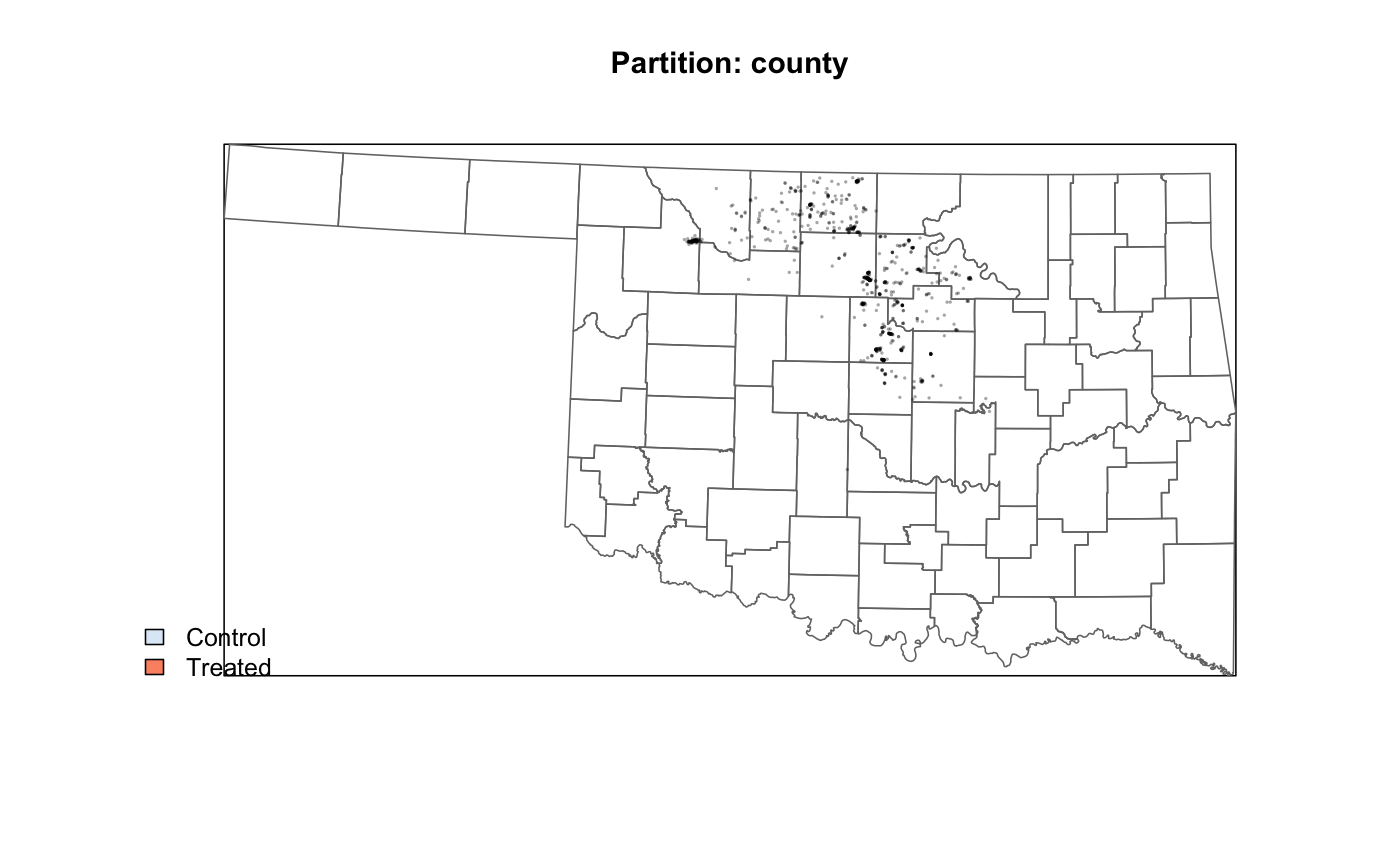
\includegraphics[width=1\linewidth,height=\textheight,keepaspectratio]{../../output/plots/partition_map_county.png}

}

\caption{\label{fig-partition-all-1}Partition maps for all partition
schemes evaluated in the run.}

\end{figure}%

\begin{figure}

\centering{

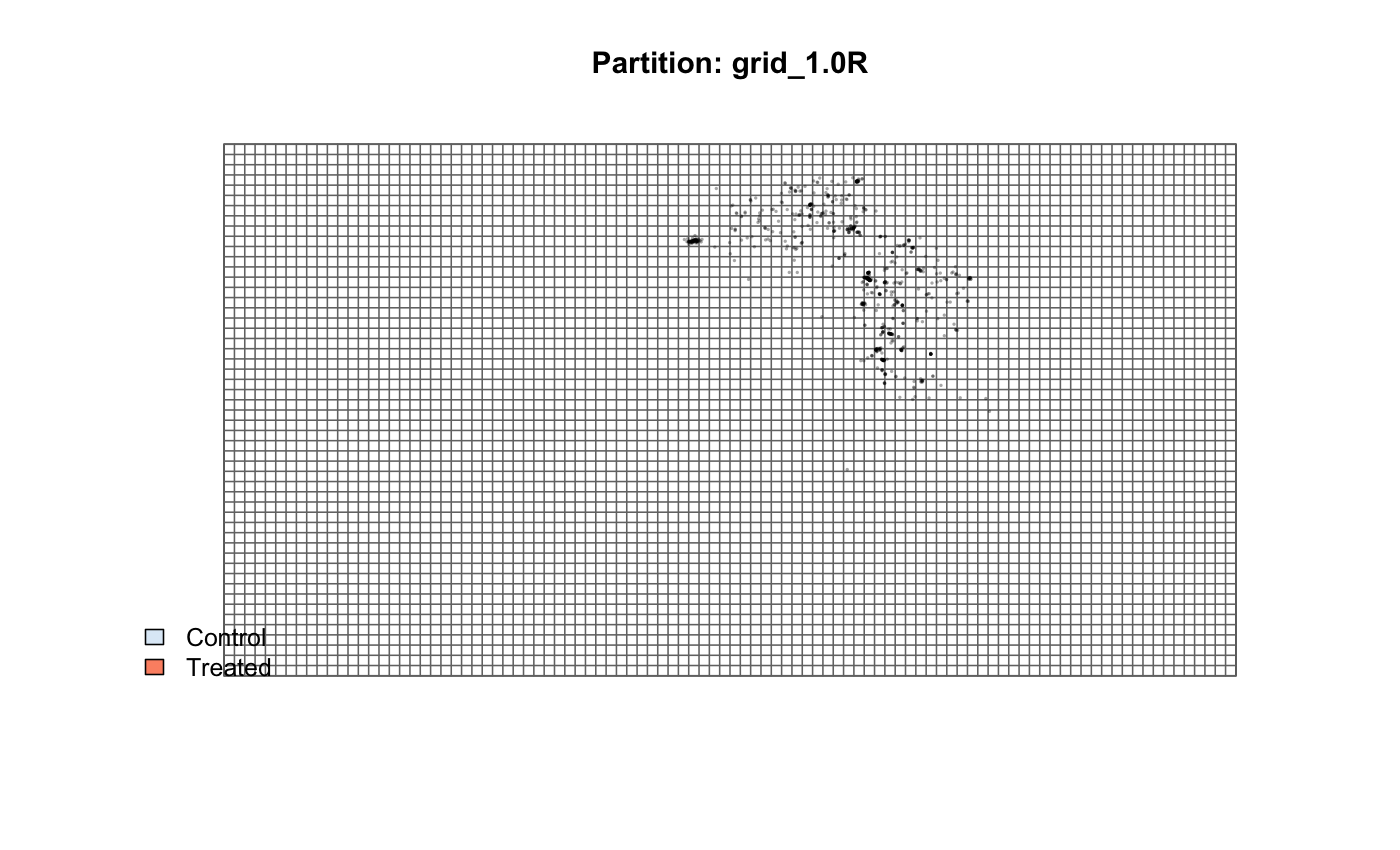
\includegraphics[width=1\linewidth,height=\textheight,keepaspectratio]{../../output/plots/partition_map_grid_1.0R.png}

}

\caption{\label{fig-partition-all-2}Partition maps for all partition
schemes evaluated in the run.}

\end{figure}%

\begin{figure}

\centering{

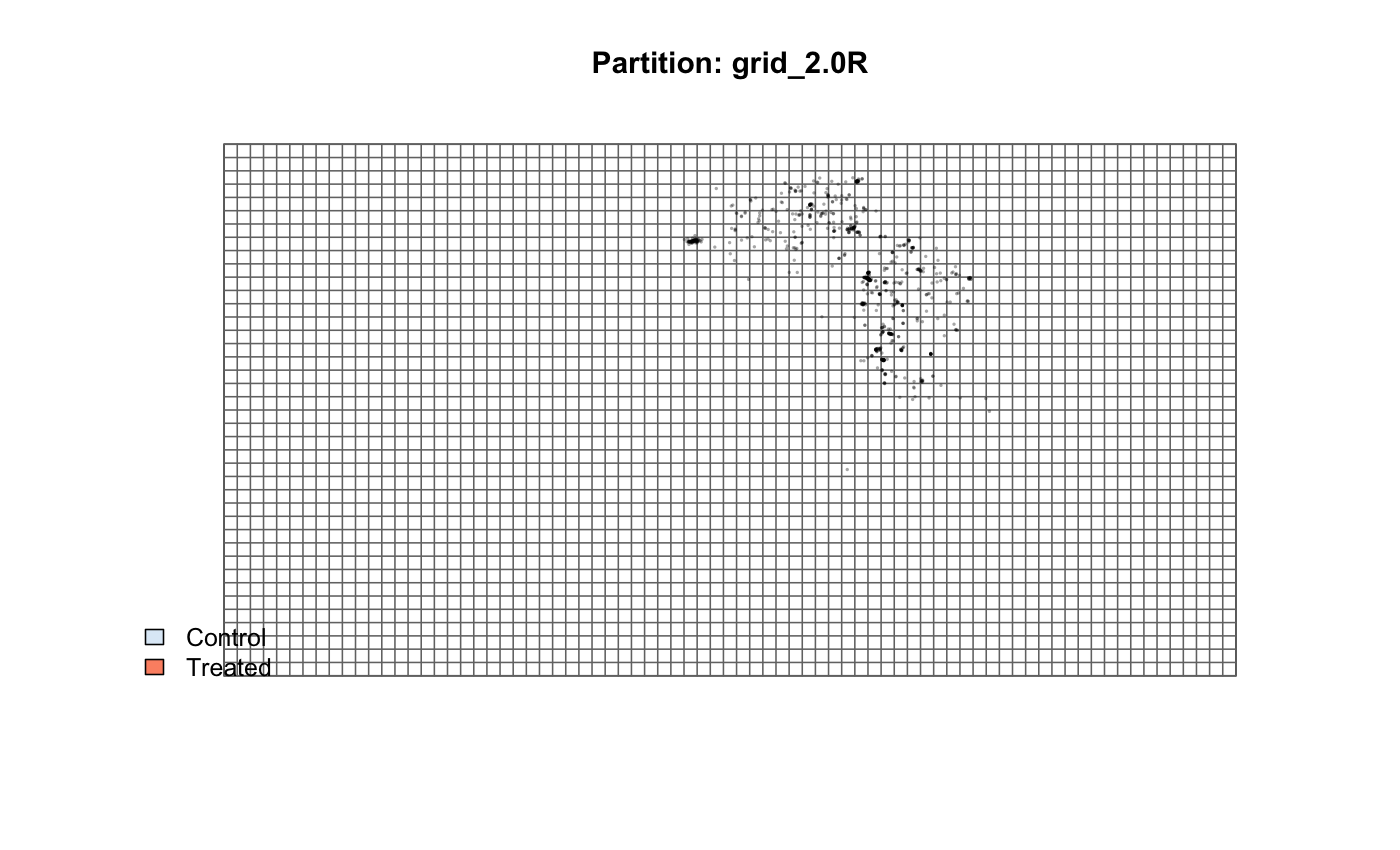
\includegraphics[width=1\linewidth,height=\textheight,keepaspectratio]{../../output/plots/partition_map_grid_2.0R.png}

}

\caption{\label{fig-partition-all-3}Partition maps for all partition
schemes evaluated in the run.}

\end{figure}%

\begin{figure}

\centering{

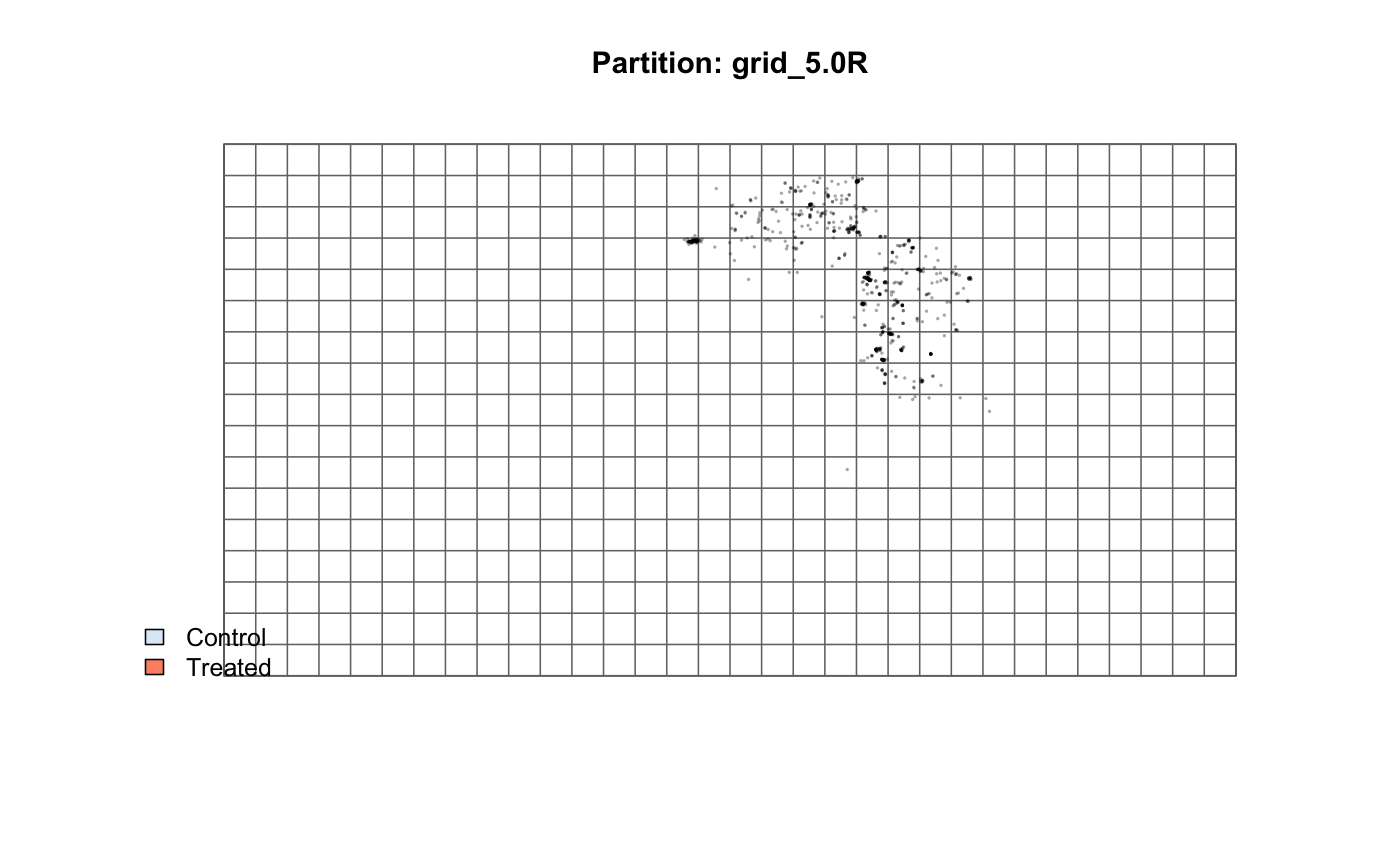
\includegraphics[width=1\linewidth,height=\textheight,keepaspectratio]{../../output/plots/partition_map_grid_5.0R.png}

}

\caption{\label{fig-partition-all-4}Partition maps for all partition
schemes evaluated in the run.}

\end{figure}%

\begin{figure}

\centering{

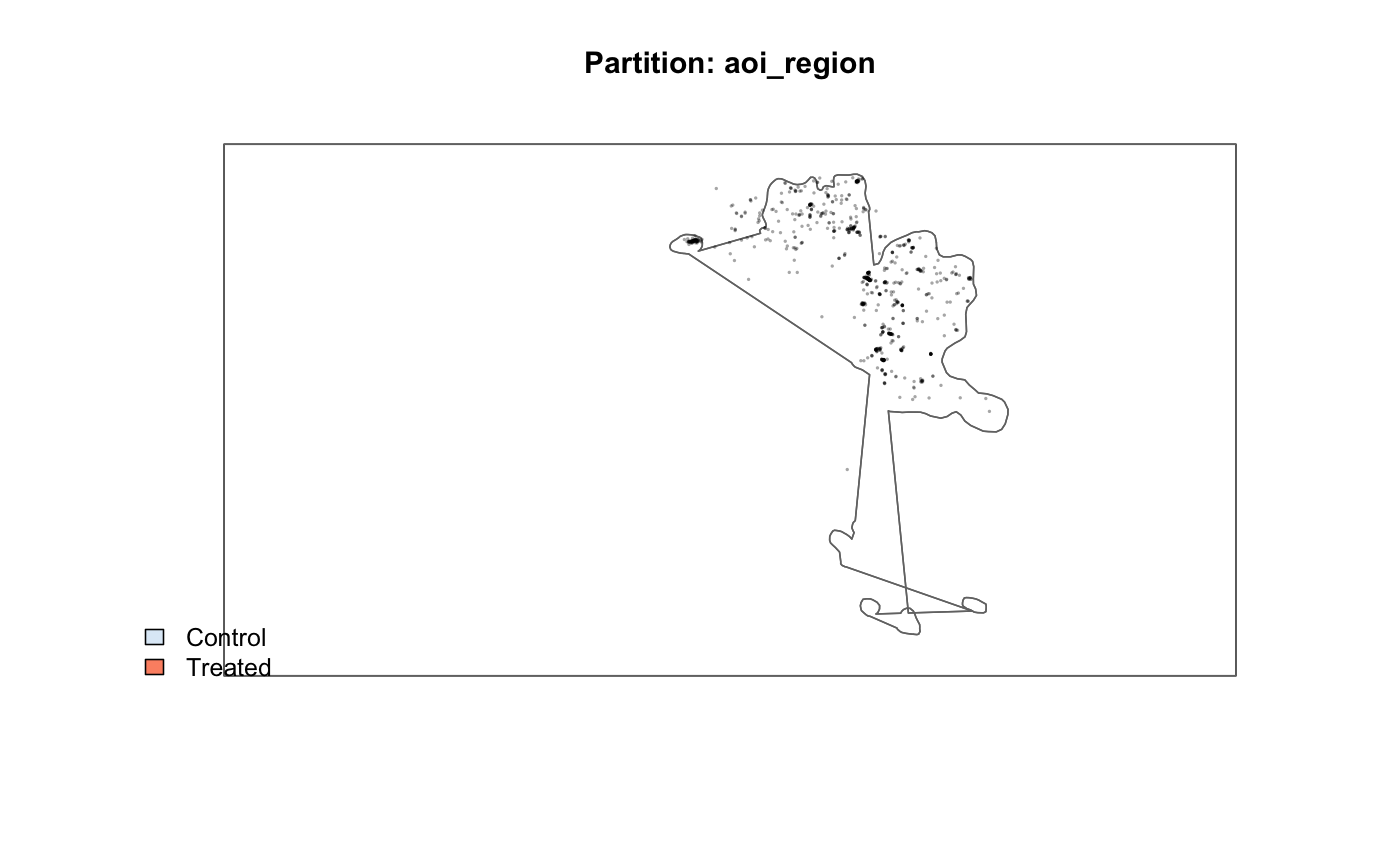
\includegraphics[width=1\linewidth,height=\textheight,keepaspectratio]{../../output/plots/partition_map_aoi_region.png}

}

\caption{\label{fig-partition-all-5}Partition maps for all partition
schemes evaluated in the run.}

\end{figure}%

\begingroup\fontsize{9}{11}\selectfont

\begin{longtable}[t]{lllcccccccccccc}

\caption{\label{tbl-partition-sensitivity}Partition comparison over 100
days: E{[}N(0){]}, E{[}N(1){]}, marginal ETAS parameters, and total
effect.}

\tabularnewline

\\
\toprule
 & Partition & Model & Tiles & Treated & Relabelled points & E[N(0)] & E[N(1)] & mu\_0 & mu\_1 & A\_0 & A\_1 & alpha\_m\_0 & alpha\_m\_1 & Total Effect\\
\midrule
1 & County & Naive Biv+KDE & 77 & 9 & 0 & 220 & 3787 & 1.8886 & 0.3697 & 0.4953 & 0.9531 & -3.1600 & 0.8654 & 3567\\
2 & County & SEM Biv+KDE & 77 & 9 & 126 & 22 & 686 & 0.0108 & 0.1481 & 1.0820 & 1.0925 & 0.5166 & 0.5996 & 663\\
9 & AOI region & Naive Biv+KDE & 2 & 1 & 0 & 44 & 896 & 0.1020 & 1.6910 & 0.9228 & 0.8459 & 0.3364 & 0.6223 & 852\\
10 & AOI region & SEM Biv+KDE & 2 & 1 & 236 & 11 & 160 & 0.0109 & 0.1624 & 1.0699 & 0.9388 & 0.4651 & 0.6409 & 149\\
3 & Grid (1x triggering range) & Naive Biv+KDE & 5096 & 440 & 0 & 25 & 870 & 0.1266 & 1.6471 & 1.0937 & 0.8316 & -0.8891 & 0.6571 & 845\\
\addlinespace
4 & Grid (1x triggering range) & SEM Biv+KDE & 5096 & 440 & 55 & 44 & 221 & 0.0241 & 0.1356 & 1.0643 & 1.0268 & 0.4285 & 0.6097 & 178\\
5 & Grid (2x triggering range) & Naive Biv+KDE & 3080 & 264 & 0 & 76 & 867 & 0.2444 & 1.7094 & 1.2453 & 0.9703 & -0.6868 & 0.3468 & 790\\
6 & Grid (2x triggering range) & SEM Biv+KDE & 3080 & 264 & 46 & 0 & 810 & 0.0020 & 0.3082 & 1.0820 & 1.0293 & 0.3423 & 0.6230 & 809\\
7 & Grid (5x triggering range) & Naive Biv+KDE & 544 & 46 & 0 & 164 & 665 & 0.9086 & 0.9850 & 0.5199 & 0.9472 & 0.3590 & 0.5251 & 501\\
8 & Grid (5x triggering range) & SEM Biv+KDE & 544 & 46 & 74 & 4 & 428 & 0.0056 & 0.1568 & 1.1406 & 1.0346 & 0.5252 & 0.6590 & 424\\
\bottomrule

\end{longtable}

\endgroup{}

\begin{figure}

\centering{

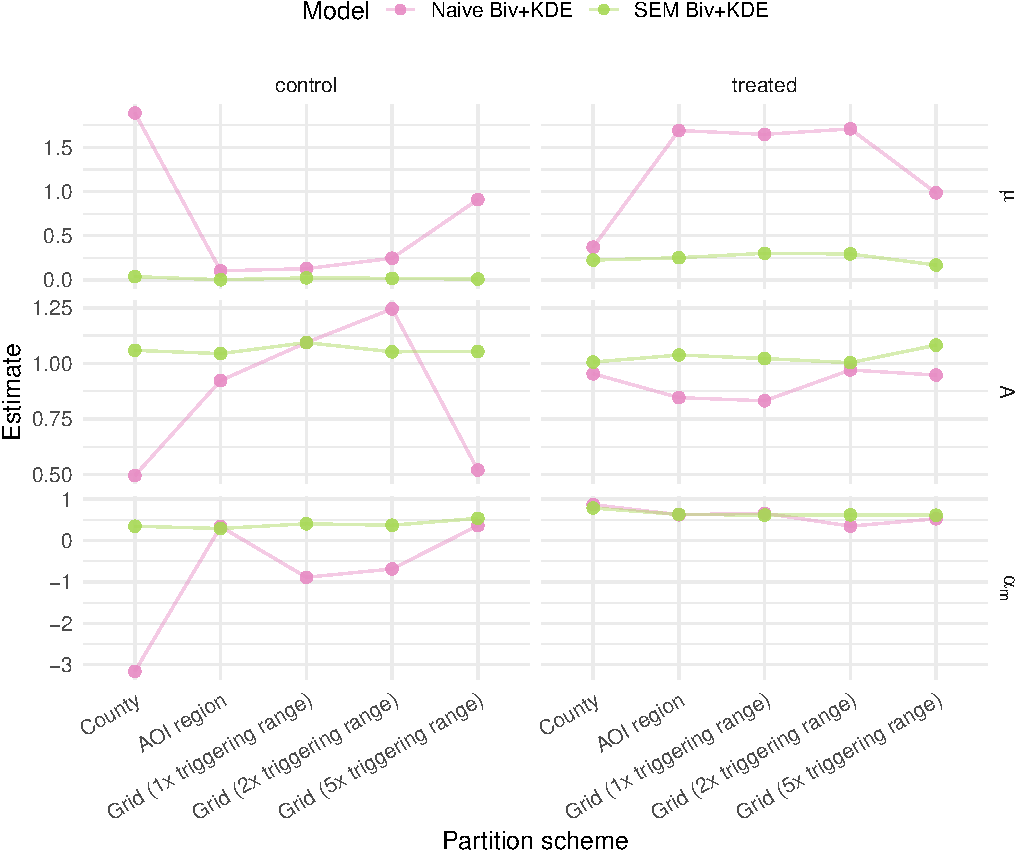
\includegraphics[width=1\linewidth,height=\textheight,keepaspectratio]{oklahoma_report_files/figure-pdf/fig-partition-params-1.pdf}

}

\caption{\label{fig-partition-params}Marginal ETAS parameters (mu, A,
alpha\_m) across partition schemes. County is highlighted to compare
against grid-based partitions.}

\end{figure}%

\begin{figure}

\centering{

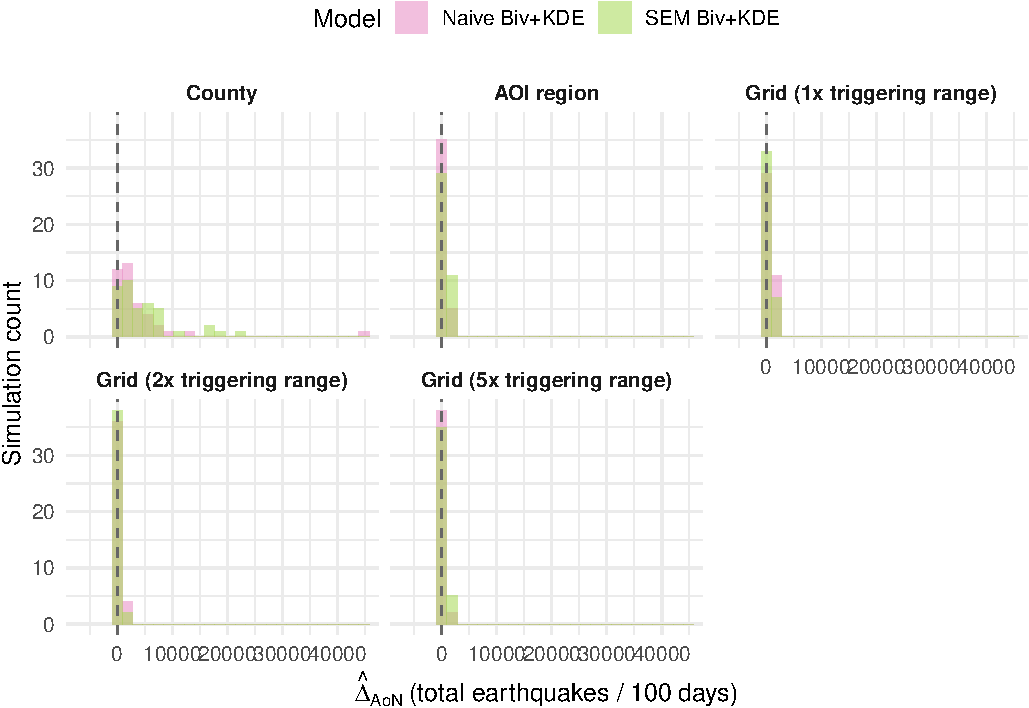
\includegraphics[width=1\linewidth,height=\textheight,keepaspectratio]{oklahoma_report_files/figure-pdf/fig-partition-ate-1.pdf}

}

\caption{\label{fig-partition-ate}Partition-sensitivity total-effect
distributions (same units and x-axis scale as Section 6.1).}

\end{figure}%

\section{Interpretation}\label{interpretation}

\textbf{Inhomogeneous background rate focus.} Fits E and F use a
spatially inhomogeneous background estimated from the first half of
control pre-treatment data. This provides an independent estimate of the
baseline seismicity pattern without using post-treatment data.

\textbf{Background contrast (inhomogeneous only).} In Fit E (naive
labels), the treated-region background rate \(\mu_1\) is 0.2\(\times\)
higher than \(\mu_0\). After SEM relabelling (Fit F), this ratio is
7.1\(\times\).

\textbf{All-or-nothing total effect (100-day horizon).}

\begin{itemize}
\tightlist
\item
  \textbf{Fit E (naive+KDE):} \(\hat\Delta_{\text{AoN}}=\) \textbf{3567}
  total earthquakes / 100 days
\item
  \textbf{Fit F (SEM+KDE):} \(\hat\Delta_{\text{AoN}}=\) \textbf{663}
  total earthquakes / 100 days
\item
  \textbf{Interpretation:} In the inhomogeneous SEM model (F), treatment
  looks \textbf{worse under treatment}; in the inhomogeneous naive model
  (E), treatment looks \textbf{worse under treatment}.
\end{itemize}

\textbf{Partition sensitivity.} The alternative partition schemes (grids
at different scales and the AOI-as-single-region partition) show how the
treatment effect estimate varies with spatial resolution. Coarser
partitions aggregate more spatial heterogeneity, while finer grids may
better capture localized effects but have fewer events per cell.

\section{Configuration}\label{configuration}

\begin{longtable}[t]{lc}

\caption{\label{tbl-config}Analysis configuration.}

\tabularnewline

\\
\toprule
Setting & Value\\
\midrule
Magnitude threshold & 2.5\\
GR β & 2.3\\
Counties (total / treated) & 77 / 9\\
SEM outer iters & 1\\
SEM inner iters & 1000\\
\addlinespace
SEM inner proposals & 20\\
SEM labellings & 30\\
SEM change factor & 0.01\\
Decode enabled & FALSE\\
Decode iterations & 200\\
\addlinespace
Fitting window (days) & 0 – 98\\
ATE simulation window (days) & 100\\
Simulation replicates & 40\\
Spatial scale D (km) & 5\\
Estimated triggering range (km) & 4.89\\
\addlinespace
Grid diameters & 4.89 km, 9.77 km, 24.43 km\\
Test mode & FALSE\\
\bottomrule

\end{longtable}

\section{References}\label{references}

\begin{itemize}
\tightlist
\item
  Ogata, Y. (1988). Statistical models for earthquake occurrences.
  \emph{JASA}, 83(401), 9--27.
\item
  Zhuang, J., Ogata, Y. \& Vere-Jones, D. (2002). Stochastic
  declustering of space-time earthquake occurrences. \emph{JASA},
  97(458), 369--380.
\item
  Helmstetter, A. \& Sornette, D. (2003). Importance of direct and
  indirect triggered seismicity in the ETAS model of seismicity.
  \emph{Geophysical Research Letters}, 30(11), 1576.
\item
  Langenbruch, C. \& Zoback, M. D. (2016). How will induced seismicity
  in Oklahoma respond to decreased saltwater injection rates?
  \emph{Science Advances}, 2(11), e1601542.
\end{itemize}

\begin{center}\rule{0.5\linewidth}{0.5pt}\end{center}

\emph{Report generated by PPDisentangle.}




\end{document}
